
% Sets the document class and font size
\documentclass[12pt]{article}
\usepackage[a4paper, margin=1in, top=0.8in, bottom=0.9in]{geometry}
\let\mathbbalt\mathbb
\usepackage[utf8]{inputenc}    % Input encoding
\usepackage[T1]{fontenc}       % Font encoding
\usepackage{fontspec}          % font encoding




% Advanced math typesetting
\usepackage{amsmath}
\usepackage{amssymb}
\usepackage{mathtools}
\usepackage{physics}


% Symbols and Text
\usepackage{bbold}     % bold font
\usepackage{ulem}      % strikethrough
\usepackage{listings}  % Source code listing
\usepackage{import}    % Importing code and other documents

% graphics
\usepackage[dvipsnames]{xcolor}
\usepackage{graphicx}
\usepackage{tikz}
\usepackage{pgfplots}
\usepackage{tcolorbox}
%\usepackage{changepage}

% figure
\usepackage{float}
\usepackage{subfigure}

\usepackage{hyperref}  % Hyperlinks in the document
\hypersetup{
    colorlinks=true,
    linkcolor=Blue,
    filecolor=red,
    urlcolor=Blue,
    citecolor=blue,
    pdftitle={Article},
    pdfauthor={Author},
}

\usepackage{xeCJK}               % Chinese, Japanese, and Korean characters
\setCJKfamilyfont{kai}{標楷體}    % Chinese font

\usepackage{subfiles}  % Best loaded last in the preamble
\usepackage{titlesec}  % fortitle

\titleclass{\subsubsubsection}{straight}[\subsection]

\newcounter{subsubsubsection}[subsubsection]
\renewcommand\thesubsubsubsection{\thesubsubsection.\arabic{subsubsubsection}}
\renewcommand\theparagraph{\thesubsubsubsection.\arabic{paragraph}} % optional; useful if paragraphs are to be numbered

\titleformat{\subsubsubsection}
  {\normalfont\normalsize\bfseries}{\thesubsubsubsection}{1em}{}
\titlespacing*{\subsubsubsection}
{0pt}{3.25ex plus 1ex minus .2ex}{1.5ex plus .2ex}

\makeatletter
\renewcommand\paragraph{
    \@startsection{paragraph}{5}{\z@}{3.25ex\@plus1ex\@minus.2ex}{-1em}{\normalfont\normalsize\bfseries}
}
\renewcommand\subparagraph{
    \@startsection{subparagraph}{6}{\parindent}{3.25ex\@plus1ex\@minus.2ex}{-1em}{\normalfont\normalsize\bfseries}
}
\def\toclevel@subsubsubsection{4}
\def\toclevel@paragraph{5}
\def\toclevel@paragraph{6}
\def\l@subsubsubsection{\@dottedtocline{4}{7em}{4em}}
\def\l@paragraph{\@dottedtocline{5}{10em}{5em}}
\def\l@subparagraph{\@dottedtocline{6}{14em}{6em}}
\makeatother

\setcounter{secnumdepth}{4}
\setcounter{tocdepth}{4}

\usepackage{fancyhdr}
\pagestyle{fancy}

\title{Note: Example for Circulation}
\date{\today}
\author{Chang-Mao Yang 楊長茂}

\begin{document}
%================================================================================================
\maketitle

\section{Line Vortex Flow}
Consider a line vortex flow in cylindrical polar coordinate $\left(r, \theta, z\right)$ with the fluid velocity vector field 
\begin{equation}
\textbf{u}
= \textbf{u}\left(\textbf{x}\right)
= \frac{k}{r} \cdot \textbf{e}_\theta,
\end{equation}
where the basis are denotes as $\textbf{e}_r$, $\textbf{e}_\theta$ and $\textbf{e}_z$. Also, in Cartesian coordinate $\left(x,y,z\right)$, the fluid velocity vector field is given by
\begin{equation}
\textbf{u}
= \textbf{u}\left(\textbf{x}\right)
= \frac{-ky}{x^2 + y^2} \cdot \textbf{e}_x + \frac{-ky}{x^2 + y^2} \cdot \textbf{e}_y,
\end{equation}
where the basis are $\textbf{e}_x$, $\textbf{e}_y$ and $\textbf{e}_z$.

\noindent\fbox{\begin{minipage}{0.99\textwidth}
Notice that the coordinates transformation between cylindrical polar coordinate and Cartesian coordinate are given by
\begin{equation}
\begin{cases}
x = r\cos\theta\\
y = r\sin\theta\\
z = z
\end{cases},\quad 
\begin{cases}
r = \sqrt{x^2 + y^2}\\
\theta = \tan^{-1} \left(y/x\right)\\
z = z
\end{cases},
\end{equation}
and the basis transformation is
\begin{equation}
\begin{cases}
\textbf{e}_r = \cos\theta \cdot \textbf{e}_x + \sin\theta \cdot \textbf{e}_y\\
\textbf{e}_\theta = -\sin\theta \cdot \textbf{e}_x + \cos\theta \cdot \textbf{e}_y \\
\textbf{e}_z = \textbf{e}_z
\end{cases},\quad 
\begin{cases}
\textbf{e}_x = \cos\theta \cdot \textbf{e}_r - \sin\theta \cdot \textbf{e}_\theta\\
\textbf{e}_y = \sin\theta \cdot \textbf{e}_r + \cos\theta \cdot \textbf{e}_\theta \\
\textbf{e}_z = \textbf{e}_z
\end{cases}
\end{equation}

\end{minipage}}

\noindent\fbox{\begin{minipage}{0.99\textwidth}
The velocity vector field in two different coordinate can be calculated by
\begin{equation}
\begin{aligned}
\textbf{u} 
&= \textbf{u}\left(\textbf{x}\right)
= \frac{k}{r} \cdot \textbf{e}_\theta 
= \frac{k}{\sqrt{x^2+y^2}} \cdot \left(-\sin\theta \cdot \textbf{e}_x + \cos\theta \cdot \textbf{e}_y\right)\\
&= \frac{k}{\sqrt{x^2+y^2}} \cdot \left(-\frac{-y}{\sqrt{x^2+y^2}} \cdot \textbf{e}_x + \frac{x}{\sqrt{x^2+y^2}} \cdot \textbf{e}_y\right)\\
&= \frac{-ky}{\sqrt{x^2+y^2}} \cdot \textbf{e}_x  + \frac{kx}{\sqrt{x^2+y^2}} \cdot \textbf{e}_y
\end{aligned}
\end{equation}
\end{minipage}}

\newpage

\section{Graph}
If we graph the velocity vector field for $k=1$, that is 
\begin{equation*}
\textbf{u}\left(x,y,z\right) = \left( \frac{-y}{x^2+y^2}, \frac{x}{x^2+y^2}, 0\right)
\end{equation*}
we get Figure \ref{fig:vec}.

\begin{figure}[h]
\centering
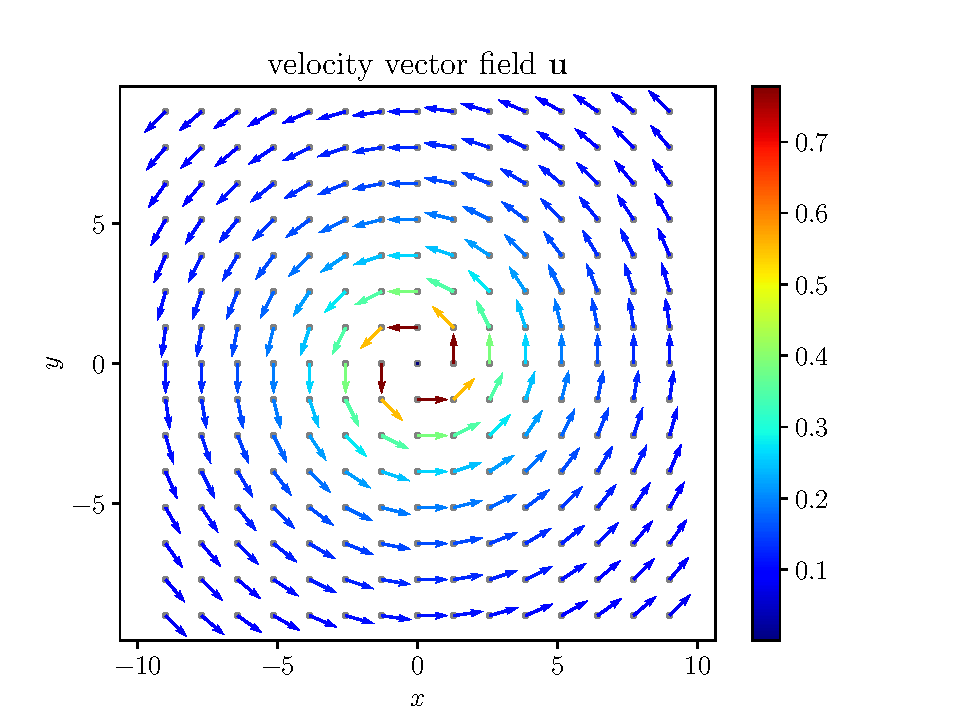
\includegraphics[width=0.69\textwidth]{img/vortex-fluid.pdf}
\caption{The length of vectors have been normalize, and the color represented the magnitude of velocity vector field $\lVert \textbf{u} \rVert$.}\label{fig:vec}
\end{figure}

\section{Vorticity}
Now, we may calculate the curl or vorticity $\xi = \nabla\times\textbf{u}$ in different coordinate system, that is
\begin{equation}
\nabla \times \textbf{u} 
= \frac{1}{r}\begin{vmatrix}
\textbf{e}_r & \textbf{e}_\theta & \textbf{e}_z \\
\partial_r & \partial_\theta & \partial_\phi \\ 
u_r & ru_\theta & u_z
\end{vmatrix}
= \frac{1}{r}\begin{vmatrix}
\textbf{e}_r & \textbf{e}_\theta & \textbf{e}_z \\
\partial_r & \partial_\theta & \partial_\phi \\ 
0 & k & 0
\end{vmatrix} = \frac{k}{r}\cdot 0 = 0
\end{equation}
and 
\begin{align}
\nabla \times \textbf{u} 
& = \begin{vmatrix}
\textbf{e}_x & \textbf{e}_y & \textbf{e}_z \\
\partial_x & \partial_y & \partial_z \\ 
u_x & u_y & u_z
\end{vmatrix}
= \begin{vmatrix}
\textbf{e}_x & \textbf{e}_y & \textbf{e}_z \\
\partial_x & \partial_y & \partial_z \\[6pt]
\displaystyle \frac{-ky}{x^2+y^2} & \displaystyle \frac{kx}{x^2+y^2} & 0
\end{vmatrix}\\
&= \left(\frac{\partial}{\partial x}\left(\frac{kx}{x^2+y^2}\right) - \frac{\partial}{\partial y}\left(\frac{-ky}{x^2+y^2}\right)\right) \textbf{e}_z\\
&= \left(\left(\frac{k\left(x^2+y^2\right) - kx \left(2x\right)}{x^2+y^2}\right) 
	+ \left(\frac{k\left(x^2+y^2\right) - ky\left(2y\right)}{x^2+y^2}\right)\right) \textbf{e}_z\\
&= \left(\frac{2k\left(x^2+y^2\right) - 2k\left(x^2 + y^2\right)}{x^2+y^2}\right)  \textbf{e}_z = 0
\end{align}
So that, the vorticity curl of line vortex fluid is zero $\xi = 0$.

\section{Circulation}
However, if we calculate the circulation of the fluid with a closed path $C$ in Cartesian coordinate
\begin{equation}
\Gamma_C 
= \oint_C \textbf{u}\cdot d\textbf{r}
\end{equation}
Notice that the $z$-component of $\textbf{u}$ is zero, the circulation is 
\begin{equation}
\Gamma_C 
= \oint_C \frac{-ky}{x^2 + y^2}\cdot dx + \frac{kx}{x^2 + y^2}\cdot dy 
= \oint_C \frac{k}{x^2+y^2}\cdot \left(xdy-ydx\right).
\end{equation}
Here, using the total differential for the $d(y/x)$, or consider a curve $(x(t),y(t))$ parametrized by $t$, we have
\begin{equation}
d\left(\frac{y}{x}\right) = \frac{xdy-ydx}{y^2}
\quad\text{or}\quad
\frac{d}{dt}\left(\frac{y(t)}{x(t)}\right) 
= \frac{\displaystyle x(t) \frac{dy(t)}{dt} - y(t) \frac{dx(t)}{dt}}{x^2(t)}.
\end{equation}
Plugin to the circulation, we have
\begin{equation}
\Gamma_C 
= k\oint_C \frac{x^2}{x^2+y^2}\cdot \left(\frac{ydx-xdy}{x^2}\right)
= k\oint_C \frac{1}{1+y^2/x^2}\cdot d\left(y/x\right).
\end{equation}
Then we easily can calculate the integral 
\begin{equation}
\Gamma_C = k\oint_C d\tan^{-1}(y/x),
\end{equation}
or in cylindrical polar coordinate $x=r\cos\theta$ and $y=r\sin\theta$
\begin{equation}
\Gamma_C = k\oint_C d\tan^{-1}(\tan\theta) = k\oint_C d\theta,
\end{equation}

\noindent\fbox{\begin{minipage}{0.99\textwidth}
\textbf{Example.}\par
If we consider a simple closed circle curve with radius $R$ parametrized by $t$, in polar coordinate we have
\begin{equation}
C: \begin{cases}
x(t) = R \cdot \cos\theta(t)\\
y(t) = R \cdot \sin\theta(t)
\end{cases},\quad R\in \mathbb{R} ,\quad \theta = [0,2\pi]
\end{equation}
the circulation is easily $\Gamma_C = 2\pi\cdot k$.
\end{minipage}}

\noindent\fbox{\begin{minipage}{0.99\textwidth}
\textbf{Remark.}
Actually, we can calculate the \textit{Winding Number} of the curve around point $0$, that is 
\begin{equation}
\Gamma_C = 2\pi \operatorname{wind}\left(C, 0\right).
\end{equation}
For more detail, see Do Carmo, M. (1976) \textit{Differential geometry of curves and surfaces},
Section 5-7, p-392.
\end{minipage}}

\noindent\fbox{\begin{minipage}{0.99\textwidth}
\textbf{Remark.}\par
In complex coordinate $z = x + iy$, also in polar coordinate, we write $z = re^{i\theta}$, then 
\begin{equation}
dz = dx + idy = e^{i\theta} dr + ire^{i\theta} d\theta.
\end{equation}
Consider 
\begin{equation}
\frac{dz}{z} 
= \frac{dx + idy}{x + iy}
= \frac{e^{i\theta} dr + ire^{i\theta} d\theta}{re^{i\theta}}
= \frac{dr}{r} + i d\theta
= d\ln r + id\theta,
\end{equation}
then integral along a closed path curve $\gamma$ in the complex plane is given by
\begin{equation}
\oint_\gamma \frac{dz}{z} = \oint_\gamma d\ln r + i \oint_\gamma d\theta = i \oint_\gamma d\theta,
\end{equation}
$r$-part vanish, since $\gamma$ is a closed curve. Now, we can rewrite the circulation for the path $\gamma$ in the complex plane, 
\begin{equation}
\Gamma_\gamma = \frac{1}{i}\oint_\gamma \frac{dz}{z}.
\end{equation}
Actually, this is a more common way to introduce \textit{Winding Number} about $z=0$, which is 
\begin{equation}
\operatorname{wind}(\gamma, 0) = \frac{1}{2\pi i}\oint_\gamma \frac{dz}{z-0}
\end{equation}
so the circulation is 
\begin{equation}
\Gamma_\gamma = \frac{1}{i} \oint_\gamma \frac{dz}{z} = \frac{1}{i} 2\pi i \operatorname{wind}(\gamma, 0) = 2\pi \operatorname{wind}(\gamma, 0).
\end{equation}



\end{minipage}}













%================================================================================================
\end{document}